\documentclass[onecolumn, draftclsnofoot,10pt, compsoc]{IEEEtran}
\usepackage{graphicx}
\usepackage{url}
\usepackage{setspace}

\usepackage{geometry}
\geometry{textheight=9.5in, textwidth=7in}

\usepackage{listings}
\usepackage{color}

\definecolor{dkgreen}{rgb}{0,0.6,0}
\definecolor{gray}{rgb}{0.5,0.5,0.5}
\definecolor{mauve}{rgb}{0.58,0,0.82}

\lstdefinestyle{php}
{
   frame=tb,
   language=PHP,
   aboveskip=3mm,
   belowskip=3mm,
   showstringspaces=false,
   columns=flexible,
   basicstyle={\small\ttfamily},
   numbers=none,
   numberstyle=\tiny\color{gray},
   keywordstyle=\color{blue},
   commentstyle=\color{dkgreen},
   stringstyle=\color{mauve},
   breaklines=true,
   breakatwhitespace=true,
   tabsize=3
}

\lstdefinestyle{javascript}
{
   frame=tb,
   language=C++,
   aboveskip=3mm,
   belowskip=3mm,
   showstringspaces=false,
   columns=flexible,
   basicstyle={\small\ttfamily},
   numbers=none,
   numberstyle=\tiny\color{gray},
   keywordstyle=\color{blue},
   commentstyle=\color{dkgreen},
   stringstyle=\color{mauve},
   breaklines=true,
   breakatwhitespace=true,
   tabsize=3
}

\lstdefinestyle{java}
{
   frame=tb,
   language=Java,
   aboveskip=3mm,
   belowskip=3mm,
   showstringspaces=false,
   columns=flexible,
   basicstyle={\small\ttfamily},
   numbers=none,
   numberstyle=\tiny\color{gray},
   keywordstyle=\color{blue},
   commentstyle=\color{dkgreen},
   stringstyle=\color{mauve},
   breaklines=true,
   breakatwhitespace=true,
   tabsize=3
}

% 1. Fill in these details
\def \CapstoneTeamName{		The Cleverly Named Team}
\def \CapstoneTeamNumber{		14}
\def \GroupMemberOne{			Omeed Habibelahian}
\def \GroupMemberTwo{			Bradley Imai}
\def \GroupMemberThree{			Dylan Tomlinson}
\def \CapstoneProjectName{		"I Heart Corvallis" Mobile Application}
\def \CapstoneSponsorCompany{	Corvallis Community Relations Office}
\def \CapstoneSponsorPerson{		Lyndi-Rae Petty}

% 2. Uncomment the appropriate line below so that the document type works
\def \DocType{		%Problem Statement
				%Requirements Document
				%Technology Review
				%Design Document
				%Progress Report
        Final Report
				}

\newcommand{\NameSigPair}[1]{\par
\makebox[2.75in][r]{#1} \hfil 	\makebox[3.25in]{\makebox[2.25in]{\hrulefill} \hfill		\makebox[.75in]{\hrulefill}}
\par\vspace{-12pt} \textit{\tiny\noindent
\makebox[2.75in]{} \hfil		\makebox[3.25in]{\makebox[2.25in][r]{Signature} \hfill	\makebox[.75in][r]{Date}}}}
% 3. If the document is not to be signed, uncomment the RENEWcommand below
\renewcommand{\NameSigPair}[1]{#1}

%%%%%%%%%%%%%%%%%%%%%%%%%%%%%%%%%%%%%%%
\begin{document}
\begin{titlepage}
    \pagenumbering{gobble}
    \begin{singlespace}
    	
\includegraphics[height=4cm]{coe_v_spot1}
        \hfill
        % 4. If you have a logo, use this includegraphics command to put it on the coversheet.
        %\includegraphics[height=4cm]{CompanyLogo}
        \par\vspace{.2in}
        \centering
        \scshape{
            \huge CS Capstone \DocType \par
            {\large\today}\par
            \vspace{.5in}
            \textbf{\Huge\CapstoneProjectName}\par
            \vfill
            {\large Prepared for}\par
            \Huge \CapstoneSponsorCompany\par
            \vspace{5pt}
            {\Large\NameSigPair{\CapstoneSponsorPerson}\par}
            {\large Prepared by }\par
            Group\CapstoneTeamNumber\par
            % 5. comment out the line below this one if you do not wish to name your team
            %\CapstoneTeamName\par
            \vspace{5pt}
            {\Large
                \NameSigPair{\GroupMemberOne}\par
                \NameSigPair{\GroupMemberTwo}\par
                \NameSigPair{\GroupMemberThree}\par
            }
            \vspace{20pt}
        }
        \begin{abstract}
        % 6. Fill in your abstract
        		This document takes a look back at the work have done on the I Heart Corvallis mobile application this past term. It recaps the purposes and goals of the project, explains our current status on the project, and details what we have left to complete. It also describes any problems that we have encountered, how they impeded our progress, and how we solved them. The document also showcases some notable pieces of code that we have recently implemented and some updated screenshots of our application and administrative website.
        \end{abstract}
    \end{singlespace}
\end{titlepage}
\newpage
\pagenumbering{arabic}
\tableofcontents
% 7. uncomment this (if applicable). Consider adding a page break.
%\listoffigures
%\listoftables
\clearpage

% 8. now you write!
\section{Introduction}
  The "I Heart Corvallis" mobile application was conceptualized by the Corvallis Community Relations office to complement their larger "I Heart Corvallis" initiative. The CCR office noticed that many OSU students do not engage much with the greater community and prefer to interact with the OSU community itself, so they started this initiative to build and promote a strong and cooperative relationship between the OSU community and the greater Corvallis community. The goal of the mobile app is to inform students about the various community events, activities, and service opportunities available to them around the community, as well as to give them an incentive to engage in these activities.
  Our client was Lyndi-Rae Petty, the Graduate Teaching Assistant at the Corvallis Community Relations office, a subset of the Office of Student Life. The development team consisted of Omeed Habibelahian, Bradley Imai, and Dylan Tomlinson. All three of us were heavily involved in nearly all aspects of the application, and we often helped each other out when one of us was stuck on a particular section of the development. It was not so much that one of us took a particular role; we were all involved in the various aspects of development and implementation, as well as in communicating updates and changes with our client. There were, however, a few aspects of the development that we each took more control of. Omeed handled more of the implementation of the administrative website, Dylan was in charge of user security on both the mobile application and the administrative website, and Bradley put in quite a bit of work on the design of the user interface.
  Our client primarily took the role of supervisor of the project. Every week we would meet with her to discuss the changes we made and new features we implemented, as well as what we had to do next, and she gave input on how she felt about our changes and anything she wanted done differently. When we needed to reach out to another organization or source for guidance or help, we would describe our situation to her, and she would take charge of reaching out to these organizations.
  \newpage

\section{Requirements Document}
  [page placeholder]\newpage
  [page placeholder]\newpage
  [page placeholder]\newpage
  [page placeholder]\newpage
  [page placeholder]\newpage
  [page placeholder]\newpage
  [page placeholder]\newpage
  [page placeholder]\newpage

\section{Design Document}
  [page placeholder]\newpage
  [page placeholder]\newpage
  [page placeholder]\newpage
  [page placeholder]\newpage
  [page placeholder]\newpage
  [page placeholder]\newpage
  [page placeholder]\newpage
  [page placeholder]\newpage
  [page placeholder]\newpage
  [page placeholder]\newpage
  [page placeholder]\newpage
  [page placeholder]\newpage

\section{Tech Review}
  [page placeholder]\newpage
  [page placeholder]\newpage
  [page placeholder]\newpage
  [page placeholder]\newpage
  [page placeholder]\newpage
  [page placeholder]\newpage
  [page placeholder]\newpage
  [page placeholder]\newpage
  [page placeholder]\newpage
  [page placeholder]\newpage
  [page placeholder]\newpage
  [page placeholder]\newpage
  [page placeholder]\newpage
  [page placeholder]\newpage
  [page placeholder]\newpage
  [page placeholder]\newpage
  [page placeholder]\newpage
  [page placeholder]\newpage
  [page placeholder]\newpage
  [page placeholder]\newpage
  [page placeholder]\newpage
  [page placeholder]\newpage
  [page placeholder]\newpage
  [page placeholder]\newpage

\section{Weekly Blog Posts}
  \subsection{Fall 2017}
    \subsubsection{Week 1}
    \subsubsection{Week 2}
    \subsubsection{Week 3}
    \subsubsection{Week 4}
    \subsubsection{Week 5}
    \subsubsection{Week 6}
    \subsubsection{Week 7}
    \subsubsection{Week 8}
    \subsubsection{Week 9}
    \subsubsection{Week 10}
  \subsection{Winter 2018}
    \subsubsection{Week 1}
    \subsubsection{Week 2}
    \subsubsection{Week 3}
    \subsubsection{Week 4}
    \subsubsection{Week 5}
    \subsubsection{Week 6}
    \subsubsection{Week 7}
    \subsubsection{Week 8}
    \subsubsection{Week 9}
    \subsubsection{Week 10}
  \subsection{Spring 2018}
    \subsubsection{Week 1}
    \subsubsection{Week 2}
    \subsubsection{Week 3}
    \subsubsection{Week 4}
    \subsubsection{Week 5}
    \subsubsection{Week 6}
    \subsubsection{Week 7}
    \subsubsection{Week 8}
    \subsubsection{Week 9}
    \subsubsection{Week 10}
  \newpage

\section{Final Poster}
  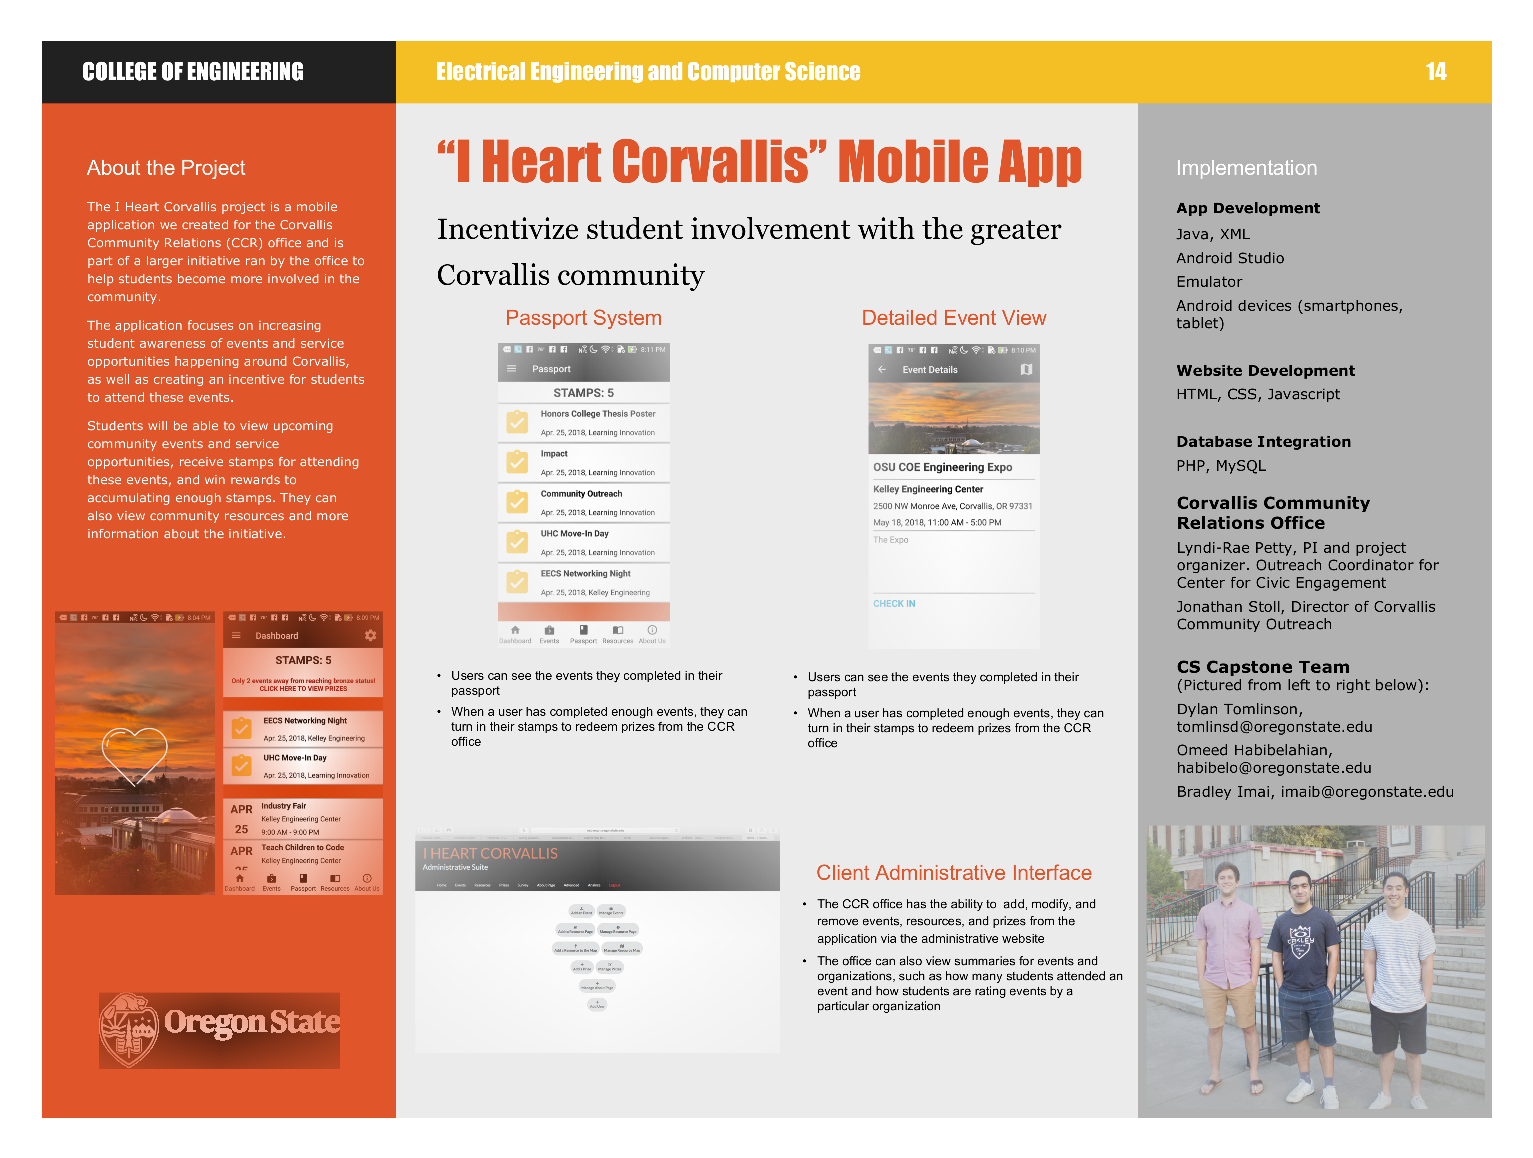
\includegraphics[height=13cm]{poster}
  \newpage

\section{Recommended Technical Resources to Learn More}
  \begin{itemize}
    \item Android Developers Website (\url{https://developer.android.com/})
    \item Derek Whiteside, Director of Web and Mobile Services at OSU
    \item Andrew Morgan, Systems Administrator, Identity and Access Management at OSU
  \end{itemize}

\section{Conclusions and Reflections}
  \subsection{Omeed}
    \subsubsection{What technical information did you learn?}
    \subsubsection{What non-technical information did you learn?}
    \subsubsection{What have you learned about project work?}
    \subsubsection{What have you learned about project management?}
    \subsubsection{What have you learned about working in teams?}
    \subsubsection{\textbf{If you could do it all over, what would you do differently?}}
  \newpage

  \subsection{Bradley}
    \subsubsection{What technical information did you learn?}
    \subsubsection{What non-technical information did you learn?}
    \subsubsection{What have you learned about project work?}
    \subsubsection{What have you learned about project management?}
    \subsubsection{What have you learned about working in teams?}
    \subsubsection{\textbf{If you could do it all over, what would you do differently?}}
  \newpage

  \subsection{Dylan}
    \subsubsection{What technical information did you learn?}
    \subsubsection{What non-technical information did you learn?}
    \subsubsection{What have you learned about project work?}
    \subsubsection{What have you learned about project management?}
    \subsubsection{What have you learned about working in teams?}
    \subsubsection{\textbf{If you could do it all over, what would you do differently?}}
  \newpage

\section{Appendix I: Essential Code Listings}
  \newpage

\section{Appendix II: Screenshots}
  \subsection{Application}
    \includegraphics[height=8cm]{splash}
    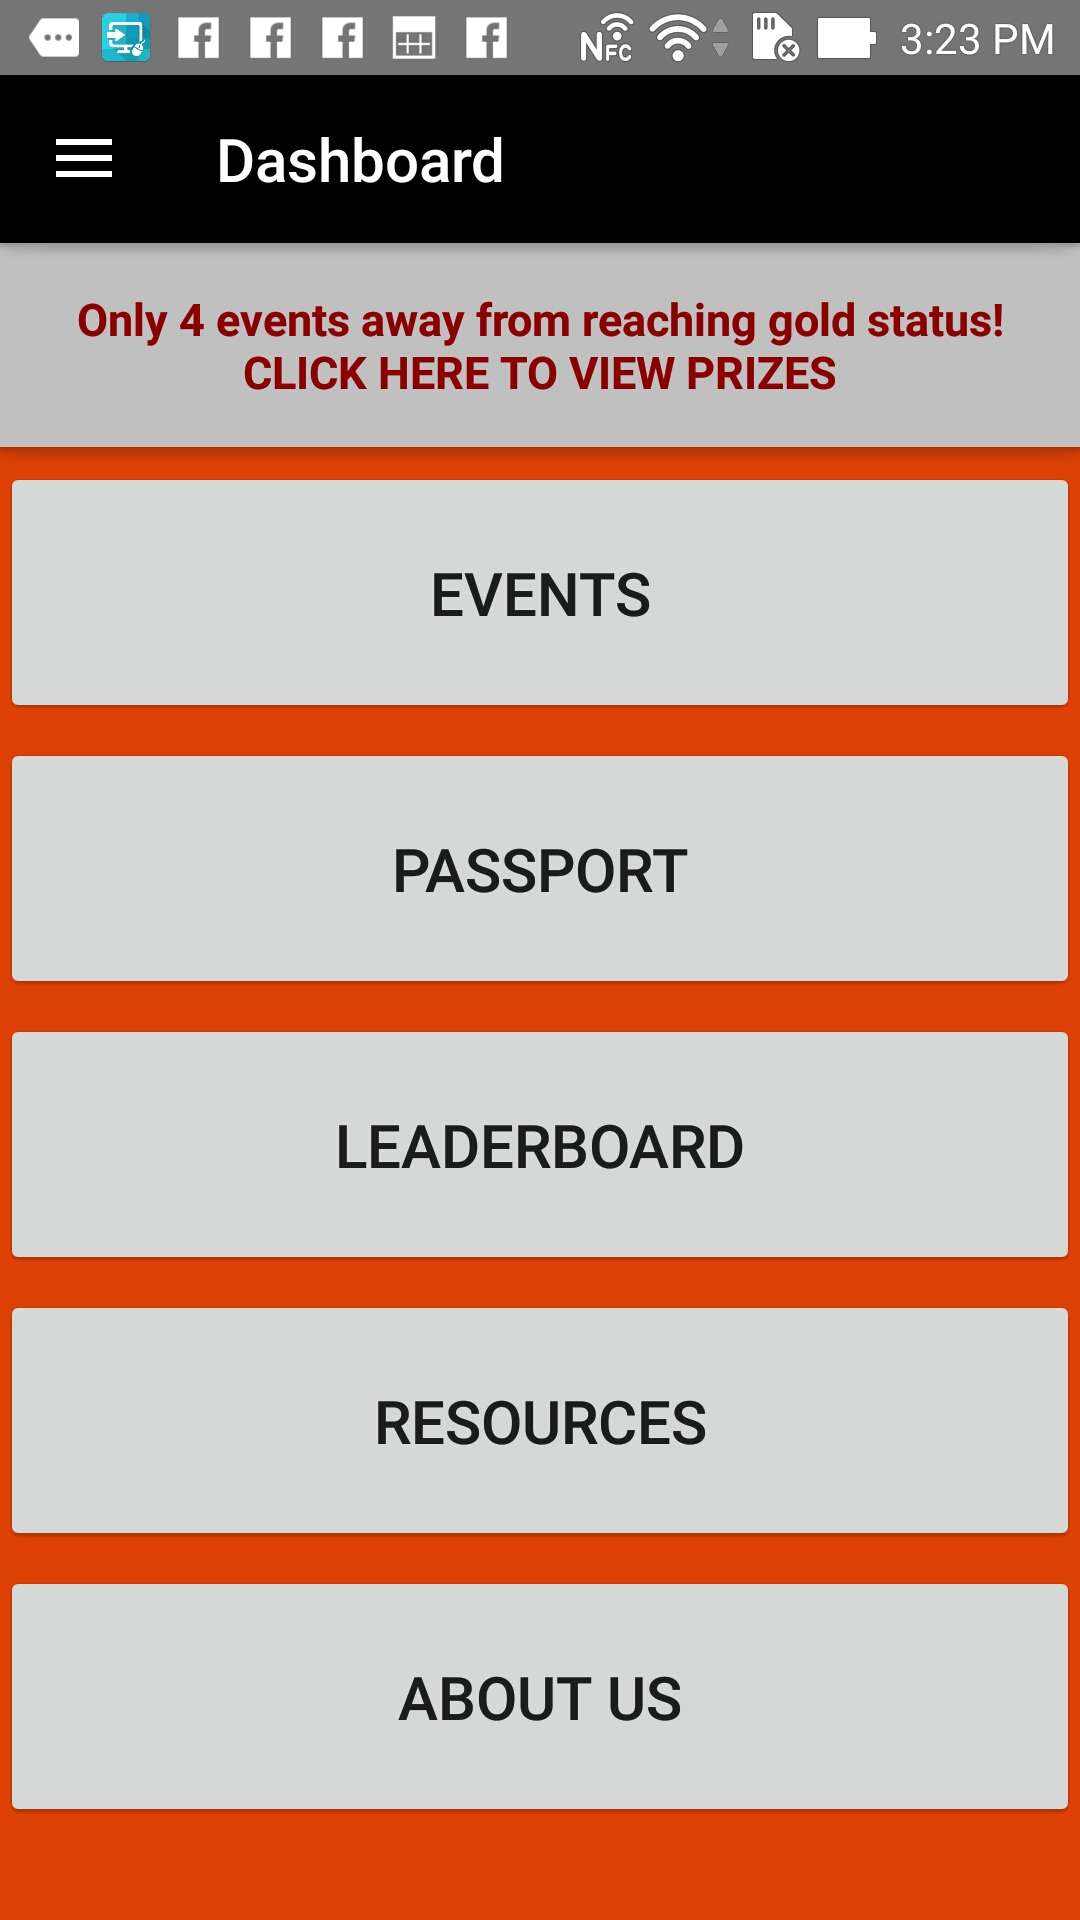
\includegraphics[height=8cm]{dashboard}
    \includegraphics[height=8cm]{eventdetail}
    
\includegraphics[height=8cm]{passport}
    \includegraphics[height=8cm]{eventmap} \\
    Top left: Splash screen \\
    Top second from left: Dashboard \\
    Top second from right: Event Detail Page \\
    Top right: Passport \\
    Bottom left: Event Map

\end{document}
